\section{Numeric Representation}

\begin{figure}
  \centering
  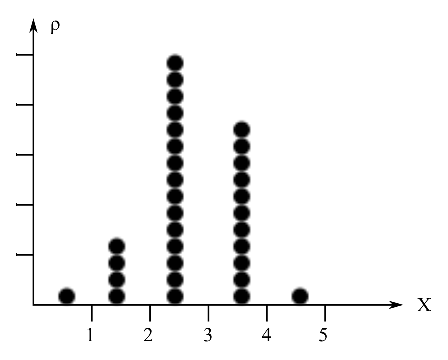
\includegraphics{Images/SkewedNormalHistogram.eps}
  \caption[Example Sample]
          {Example Sample}
  \label{fig:SkewedNormalHistogram2}
\end{figure}

\begin{figure}
  \centering
  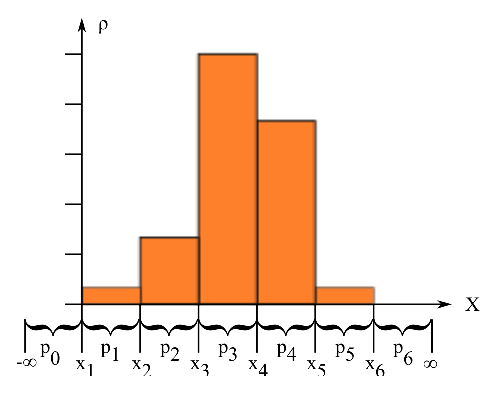
\includegraphics{Images/ArbitraryHistogram.eps}
  \caption[1D Numeric Random Variable]
          {1D Numeric Random Variable}
  \label{fig:ArbitraryHistogram}
\end{figure}

Given a sample of a random variable and a partition of the support space as in figure \ref{fig:SkewedNormalHistogram2} a histogram forms a natural summary. In RICO, a method of representing a one dimensional continuous random variable numerically is suggested in figure \ref{fig:ArbitraryHistogram}. Since random variables may be both discrete and continuously distributed at the same time a pair of parallel arrays is used programmatically,
\begin{align*}
X \sim \begin{cases}
    X_c = \begin{cases}
    (x_0 = -\infty, x_1, x_2, ..., x_n, x_{n+1} = \infty)\\
    (p_0, p_1, ..., p_n, 0)
    \end{cases}\\
    X_d = \begin{cases}
    (y_1, y_2, ..., x_m)\\
    (q_1, q_2, ..., q_m)
    \end{cases}
  \end{cases}
\end{align*}
where
\begin{align*}
-\infty < x_1 < ... < x_n < \infty
\end{align*}
The endpoints for the continuously distributed portion of $X$, $X_c$, are assumed to be $\pm \infty$ with $n$ partition endpoints between. The $p_i$ values are defined as
\begin{align*}
p_i := \begin{cases}
  P(x_i < X_c < x_{i+1}) & \text{ if } i \in \{1, ..., n-1\}\\
  P(X_c < x_1) & \text{ if } i = 0\\
  P(x_n < X_c) & \text{ if } i = n+1
  \end{cases}
\end{align*}
and the $q_j$ values are defined as
\begin{align*}
q_j := P(X_d = y_j) \text{ for } j \in \{1, ..., m\}
\end{align*}

For an example of RICO in action, let $X \sim N(0,1)$ numerically represented. New random variables such as $e^X$ and $X^{1.25}$ can be created and graphed, see table \ref{fig:OneDimFunction}. The code used to generate the graphs is

\begin{lstlisting}
X = NormalNumeric(0,1,1000)
Plot(exp(X))
Plot(X**1.25)
\end{lstlisting}


\begin{table}
\begin{center}
\begin{tabular}{cc}
$X$ & $e^X$\\
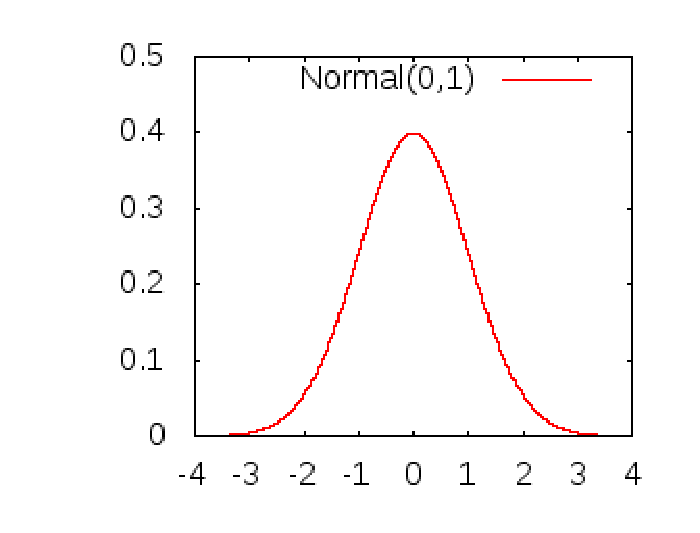
\includegraphics[width=2in]{Images/NormalDSN.eps} &
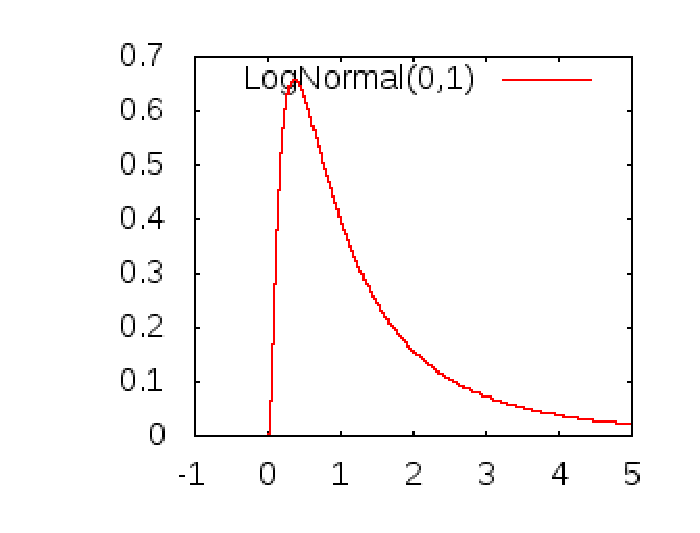
\includegraphics[width=2in]{Images/LogNormalDSN.eps} \\
$X$ & $X^{1.25}$\\
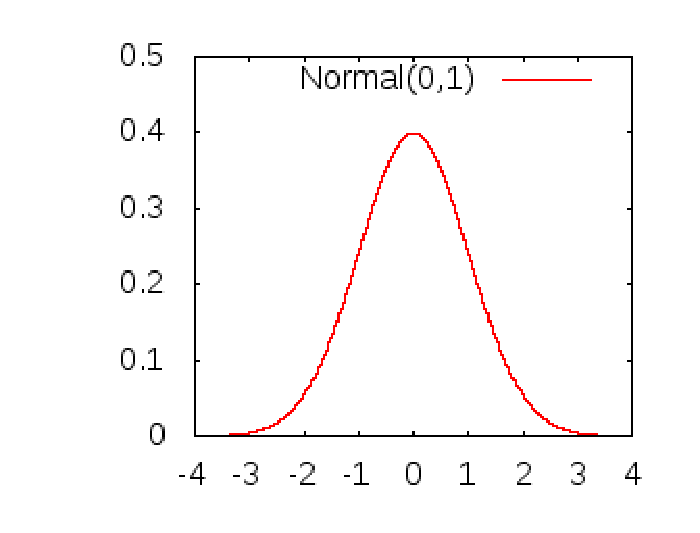
\includegraphics[width=2in]{Images/NormalDSN.eps} &
\includegraphics[width=2in]{Images/PowerNormalDSN.eps} \\
\end{tabular}
\end{center}
\caption[Standard Normal $X$, $e^X$, $X^{1.25}$]
        {Standard Normal $X$, $e^X$, $X^{1.25}$}
\label{fig:OneDimFunction}
\end{table}

\begin{figure}
  \centering
  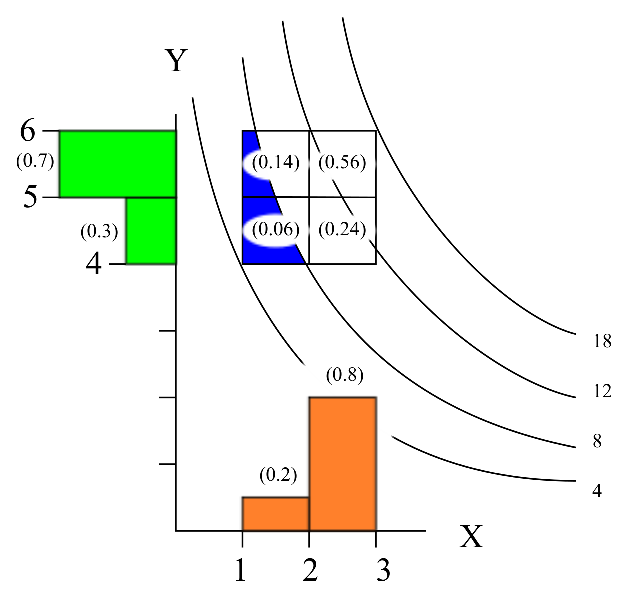
\includegraphics[width=3in]{Images/AxB_partitioned.eps}
  \caption[Piecewise Continuous X times Y]
          {Piecewise Continuous X times Y}
  \label{fig:AxB_Partitioned}
\end{figure}

Illustrative example of multiplication of two piecewise continuous random variables $X$ and $Y$.  Referring to figure \ref{fig:AxB_Partitioned}, the following conditions hold for $X$ and $Y$,
\begin{align*}
P(1 < X < 2) = 0.2 && P(2 < X < 3) = 0.8\\
P(4 < Y < 5) = 0.3 && P(5 < Y < 6) = 0.7
\end{align*}
and the probability densities are super-imposed on the joint density distribution of $(X,Y)$. For illustrative purposes a partition of the $XY$ random variables is chosen as $(4,8,12,18)$ to coincide with the corners of the non-zero probability density region of $(X,Y)$. Each partition endpoint $\{4,8,12,18\}$ corresponds to an iso-probability level curve identified in the figure \ref{fig:AxB_Partitioned}. Notice that in the case of multiplication the level curves are hyperbolas. To compute the numeric random variable $XY$ given the partition $(4,8,12,18)$, calculate the area between level curves within joint probability rectangles. In particular, to compute $P(4 < XY < 8)$ one must find the fractional area of each of the two shaded rectangles multiplied by the probability contained in each such rectangle. The probability of the two shaded rectangles is $0.14 + 0.06 = 0.2$. To compute the probability of the shaded area using RICO involves forcing the particular partition shown in the figure as follows,
\begin{lstlisting}
X = ContinuousNumeric((1,2,3),(0.2,0.8,0))
Y = ContinuousNumeric((4,5,6),(0.3,0.7,0))
Y.getNumericRandomVariable().force_partition((4,8,12,18))
X*Y
#()
#(4.0(0.11130904824004995)8.0(0.3565452412002493)12.0(0.5321457105597007)18.0,)
\end{lstlisting}

According to RICO the results of the above numerical example are
\begin{align*}
P(4 < XY < 8) \approx 11\% && P(8 < XY < 12) \approx 36\% && P(12 < XY < 18) \approx 53\%
\end{align*}

\begin{figure}
  \centering
  \includegraphics[width=3in]{Images/N53xN11.eps}
  \caption[N(5,3) x N(1,1)]
          {N(5,3) x N(1,1)}
  \label{fig:N53xN11}
\end{figure}

A larger example of multiplication is $XY$ where $X \sim N(5,3), Y \sim N(1,1)$. The listing follows as the plot is shown in figure \ref{fig:N53xN11}.
\begin{lstlisting}
X = Normal(5,3)
Y = Normal(1,1)
XY = X*Y
Plot().xrange(-20,30).plot(XY).show()
\end{lstlisting}

Similarly, division of two numeric random variables, this time in one line of code with the result shown in figure \ref{fig:N73_N11} which happens to be multi-modal. 
\begin{lstlisting}
Plot().xrange(-20,30).plot(Normal(7,3)/Normal(1,1)).show()
\end{lstlisting}

\begin{figure}
  \centering
  \includegraphics[width=3in]{Images/N73_N11.eps}
  \caption[N(7,3) / N(1,1)]
          {N(7,3) / N(1,1)}
  \label{fig:N73_N11}
\end{figure}

\section{Correlation}
Consider the example in figure \ref{fig:Product_Power} without preperatory remarks.
\begin{table}
\begin{center}
\begin{tabular}{cc}
$X*X$ & $X^2$\\
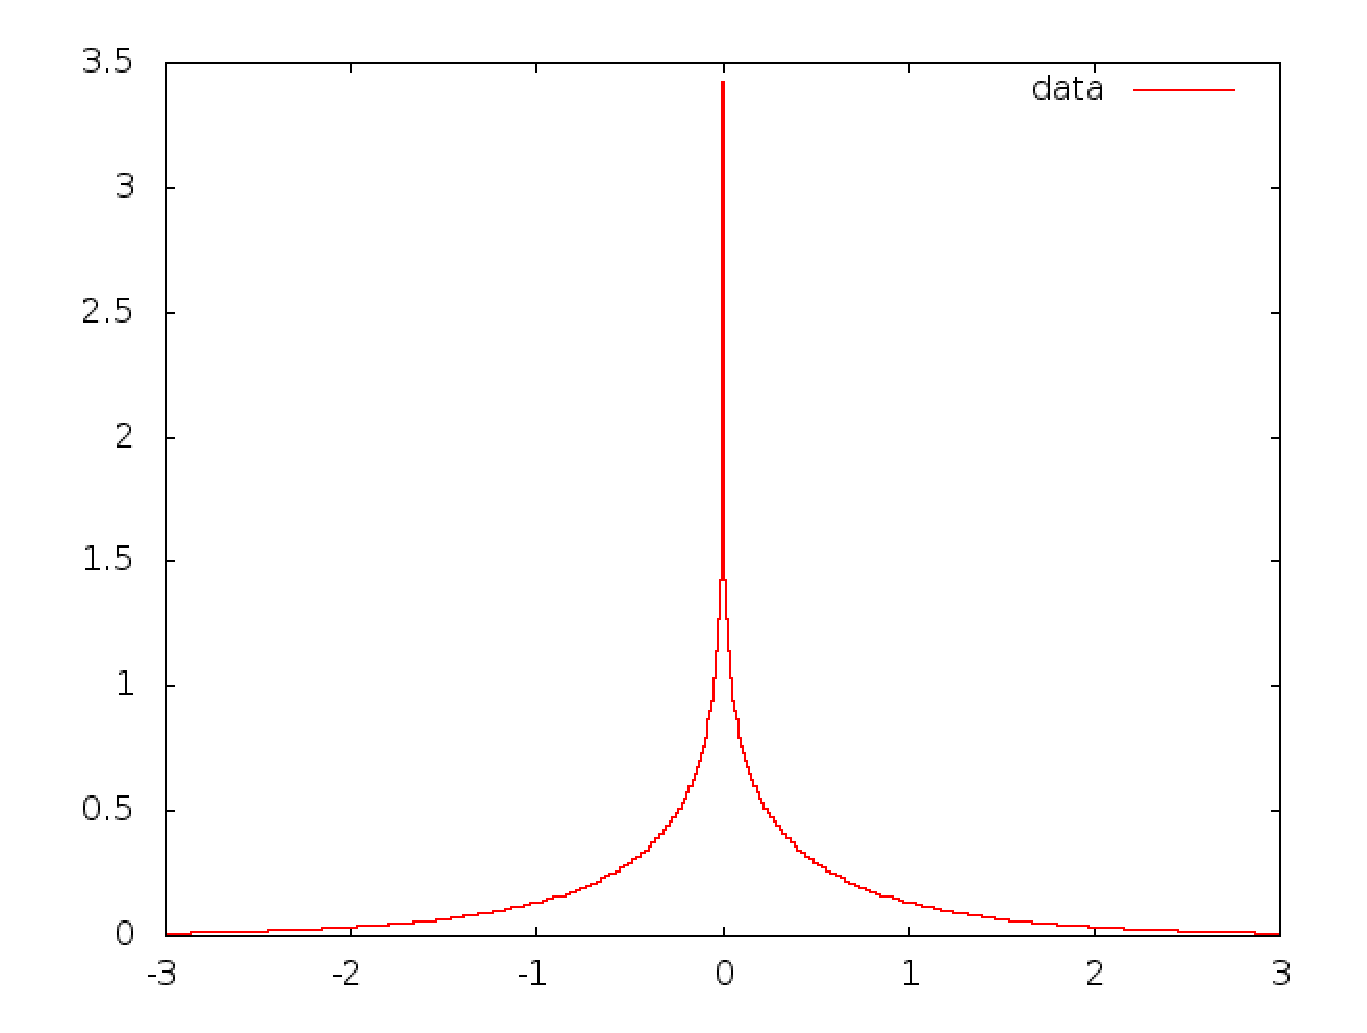
\includegraphics[width=2in]{Images/N01xN01.eps} &
\includegraphics[width=2in]{Images/N01xx2.eps} \\
\end{tabular}
\end{center}
\caption[Standard Normal $X*X$ versus $X^2$]
        {Standard Normal $X*X$ versus $X^2$}
\label{fig:Product_Power}
\end{table}

The issue in figure \ref{fig:Product_Power} is that RICO needs to understand that two references to the same underlying variable are $100\%$ correlated. When RICO is asked to compute $X^2$ there is no confusion, but $X*X$, without correlation tracking appears as the product of two independent copies of $X$.

Within the context of an algorithmic model with some random variable inputs intermediate variables are created and mixed with other intermediate variables such that partially correlated expressions are possible,
\begin{align*}
X + XY\\
X + Y/X
\end{align*}
Assuming that $X \perp Y$ the multiplication $XY$ is between independent random variables and is computable is detailed in the previous section. The sum in $X + XY$ is not between independent random variables. Fortunately RICO is equipped with a symbolic processing engine so that the expression $X+XY$ will be factored into $X(1+Y)$. This expression is computable as a sequence of operations. The expression $1+Y$ is independent of $X$ so the product $X(1+Y)$ is between independent random variables. 

\begin{figure}
  \centering
  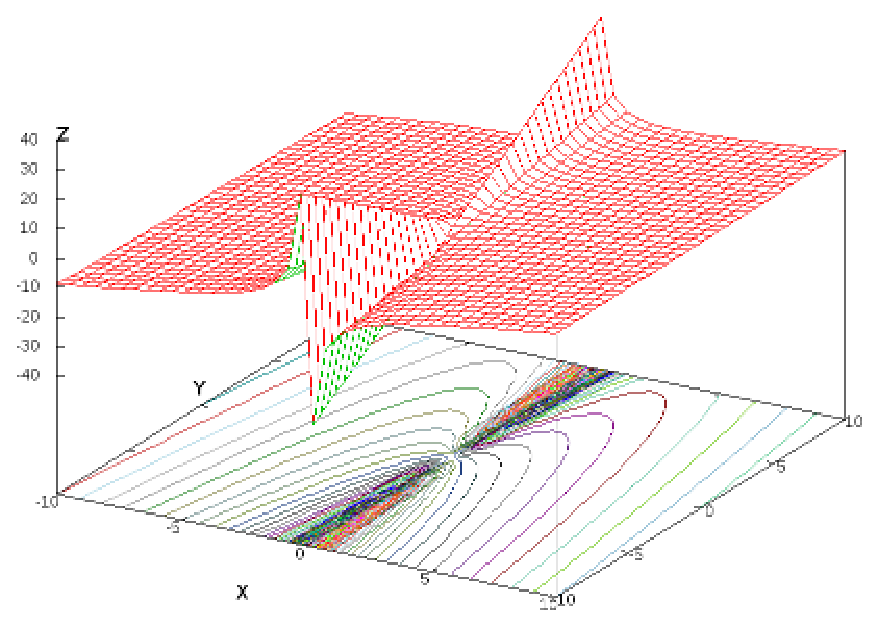
\includegraphics[width=3in]{Images/XpY_X.eps}
  \caption[X + Y/X]
          {X + Y/X}
  \label{fig:XpY_X}
\end{figure}

The expression $X+Y/X$ is not decomposible into a sequence of operations between independent random variables. In such a case the iso-probability level curves are more complicated than the hyperbolas found in the multiplication case. The level curves for a particular partition of $Z = X+Y/X$ are shown in figure \ref{fig:XpY_X}.

In the case of $Z = X + Y/X$, the partitions of $X$ and $Y$ for a partition of the joint $(X,Y)$ space. A subset of the iso-probability level curves associated with the partition of $Z$ are approximated within each $(X,Y)$-partition rectangle bounded by $(x_0, y_0)$ and $(x_1, y_1)$, relatively indexed, by approximating the supported probability surface $f$ with a bilinear function of $X$ and $Y$ as
\begin{align*}
f(x,y) = axy + bx + cy + d
\end{align*}
where the coefficients $(a,b,c,d)$ are
\begin{align*}
\begin{pmatrix}a\\b\\c\\d\end{pmatrix} = 
  \begin{pmatrix}x_0 y_0 & x_0 & y_0 & 1\\
                 x_1 y_0 & x_1 & y_0 & 1\\
                 x_0 y_1 & x_0 & y_1 & 1\\
                 x_1 y_1 & x_1 & y_1 & 1
  \end{pmatrix} ^ {-1} 
  \begin{pmatrix}
    f(x_0, y_0)\\f(x_1, y_0)\\f(x_0, y_1)\\f(x_1, y_1)
  \end{pmatrix}
\end{align*}
An iso-probability level curve is then a function $y(x | z)$ for a given partition endpoint $z$ as
\begin{align*}
y(x | z) = \frac{z - d - bx}{ax + c}
\end{align*}
A necessary step is to compute the fraction of each $(X,Y)$-partition rectangle intersected each given $Z$-partition interval. The bilinear approximation admits the following closed form solution,
\begin{align*}
\int y(x | z) \; dx = \frac{log(ax+x)(az - ad + bc)-abx}{a^2} + const
\end{align*}

\begin{figure}
  \centering
  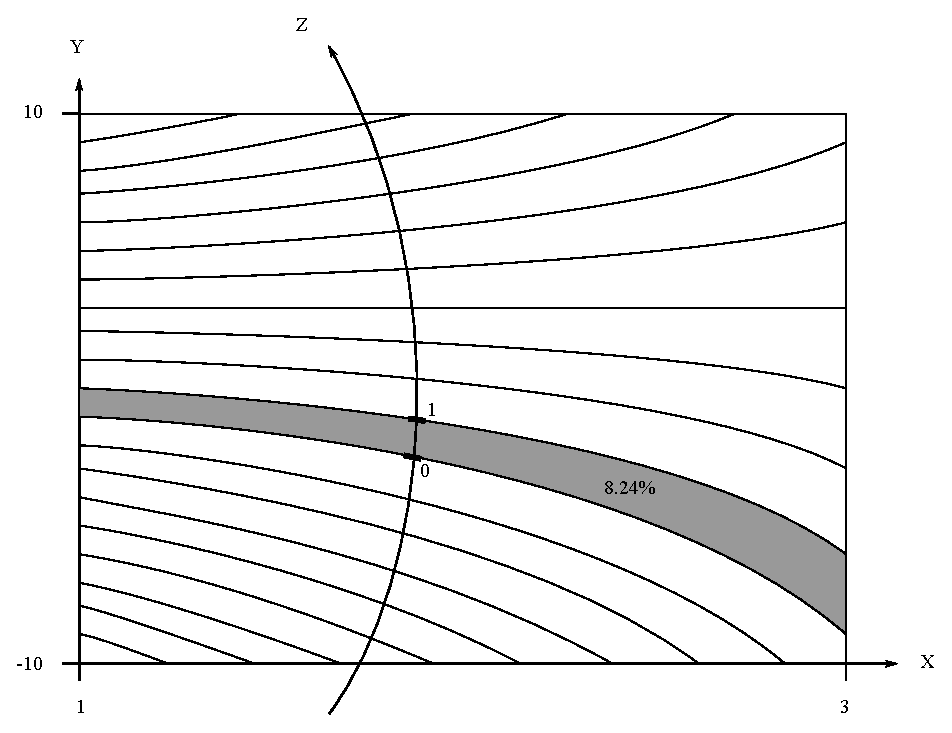
\includegraphics[width=3in]{Images/XpY_Zrectangle.eps}
  \caption[A partition element of X + Y/X with level curves]
          {A partition element of X + Y/X with level curves}
  \label{fig:XpY_Zrectangle}
\end{figure}

As a numerical example suppose $X$ has a partition element bounded by $\{1,3\}$ and similarly $Y$ has a partition element bounded by $\{-10,10\}$. If $Z$ has a partition element bounded by $\{0,1\}$ then figure \ref{fig:XpY_Zrectangle} shows that appoximately $8.25\%$ of the probability represented by this partition rectangle is allocated to the $(0,1)$ partition element of $Z$. The resulting probability distribution for $Z$ is shown in figure \ref{fig:XpY_X_Z}.

\begin{figure}
  \centering
  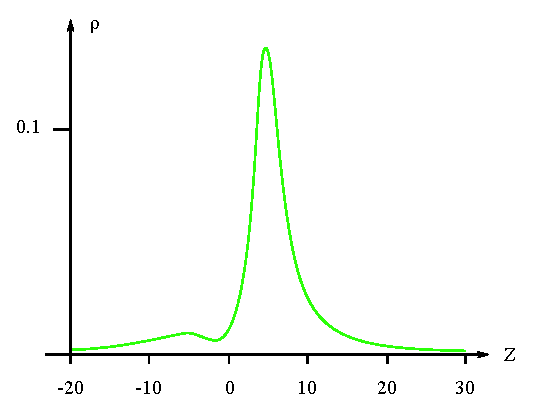
\includegraphics[width=3in]{Images/XpY_X_Z.eps}
  \caption[$X+Y/X$ where $X\sim N(5,3), Y \sim N(1,1)$]
          {$X+Y/X$ where $X\sim N(5,3), Y \sim N(1,1)$}
  \label{fig:XpY_X_Z}
\end{figure}

